%%%%%%%%%%%%%%%%%%
\section{基于后期融合最大化的多视图聚类方法}


\begin{frame}
    \frametitle{我们的方法:MVC-LFA(Late Fusion Alignment)}
    \begin{itemize}
        \item 我们提出了基于后期融合最大化的多视图方法(ijcai-19)
    \end{itemize} 
    \begin{figure}
        \includegraphics[width=0.9\textwidth]{figures/model3.jpg} 
    \end{figure}          
\end{frame}

\begin{frame}
    \frametitle{MVC-LFA}
    \begin{itemize}
        \item 考虑$k$-means的优化目标:
\begin{equation}\label{LFA 1}
\begin{split}
\min\nolimits_{\mathbf{H}^*}\;&\;\mathrm{Tr}(\mathbf{X} \mathbf{X}^{\mathrm{ T }}) - \mathrm{Tr} ( {\mathbf{H}^*}^{\mathrm{ T }} \mathbf{X} \mathbf{X}^{\mathrm{ T }} \mathbf{H}^*),\\
s.t. &\;  \bf{H}^* \in \mathbb{R}^{\mathit{n}\times \mathit{k}}, {\mathbf{H}^*}^{ \mathrm{ T }}\mathbf{H}^* = \mathbf{I}_k,
\end{split}
\end{equation}
         \item $\mathbf{X}$ 和 $\mathbf{H}^*$分别是数据矩阵和聚类结果矩阵。我们通过对 Eq.(\ref{LFA 1})中的$\mathbf{X} \mathbf{X}^{\mathrm{ T }}$进行SVD分解来得到最后的划分矩阵 $\mathbf{H}^*$。
         \item  当对应到多视图数据$\mathbf{X}= \sum_{p=1}^m \beta_p \mathbf{H}_p \mathbf{W}_p$时,优化过程很复杂。
    \end{itemize}   
      
\end{frame}

\begin{frame}
    \frametitle{MVC-LFA}
    \begin{itemize}
        \item 贡献一:我们首先证明了 Eq.(\ref{LFA 1})中的优化目标等价于最大化后期融合之间的对齐$\mathrm{Tr} ({\mathbf{H}^*}^{ \mathrm{ T }} \mathbf{X})$。
        \item
 \begin{proof}
因为$\mathbf{P} = {\mathbf{H}^*}^{ \mathrm{ T }} \mathbf{X}$,我们可以得到 $\mathrm{Tr}^2 ({\mathbf{H}^*}^{ \mathrm{ T }} \mathbf{X}) \leq k \cdot  \mathrm{Tr}({\mathbf{H}^*}^{ \mathrm{ T }} \mathbf{X} \mathbf{X}^{\mathrm{ T }}{\mathbf{H}^*} )$.
因此,
$
\mathrm{Tr}(\mathbf{X} \mathbf{X}^{\mathrm{ T }}) - \mathrm{Tr} ( {\mathbf{H}^*}^{\mathrm{ T }} \mathbf{X} \mathbf{X}^{\mathrm{ T }} \mathbf{H}^*) \leq 2k - \mathrm{Tr} ( {\mathbf{H}^*}^{\mathrm{ T }} \mathbf{X} \mathbf{X}^{\mathrm{ T }} \mathbf{H}^*) \leq  2k - \frac{1}{k} \mathrm{Tr}^2 ({\mathbf{H}^*}^{ \mathrm{ T }} \mathbf{X}).
$
\end{proof}
    \end{itemize} 
    
      
\end{frame}

\begin{frame}
    \frametitle{MVC-LFA优化目标}
    \begin{itemize}
        \item 根据上面的结论,我们提出了一种简单但是高效的多视图聚类算法:
        \item \begin{equation}
\label{LFA 2}
\begin{split}
\;&\;\max\nolimits_{\mathbf{H}^*,\left\{\mathbf{W}_p\right\}_{p=1}^m,\beta} \mathrm{Tr} ({\mathbf{H}^*}^{ \mathrm{ T }} \mathbf{X}) + \lambda \mathrm{Tr}({\mathbf{H}^*}^{ \mathrm{ T }} \mathbf{M}),\\
\;&\; s.t.\;{\mathbf{H}^*}^{ \mathrm{ T }}\mathbf{H}^* = \mathbf{I}_k, \mathbf{{W}}_p^{ \mathrm{ T }}\mathbf{W}_p = \mathbf{I}_k,\\
\;&\;\sum\nolimits_{p=1}^m {\beta_{p}}^2 = 1, \beta_{p} \geq 0,\mathbf{X}= \sum\nolimits_{p=1}^m \beta_p \mathbf{H}_p \mathbf{W}_p,
\end{split}
\end{equation}
    \end{itemize} 
  
      
\end{frame}

\begin{frame}
    \frametitle{MVC-LFA}
    \begin{itemize}
        \item 贡献二:我们从理论上说明了算法的收敛性:
        \item 
\begin{proof}
因为我们的优化方法采用了轮替优化法,当中每一步都是最优解,所以我们只需证明我们的算法有一个上界即可。注意到$ \forall p,q,\,\mathrm{Tr}[{(\beta_{p}\mathbf{H}_p\mathbf{W}_p)}^{\mathrm {T}} (\beta_{q}\mathbf{H}_q\mathbf{W}_q)]\leq  \mathrm{Tr}[{(\mathbf{H}_p\mathbf{W}_p)}^{\mathrm {T}} (\mathbf{H}_q\mathbf{W}_q)] \leq \frac{1}{2} (\mathrm{Tr} [{(\mathbf{H}_p\mathbf{W}_p)}^{\mathrm {T}} {(\mathbf{H}_p\mathbf{W}_p)}]  + \mathrm{Tr} [{(\mathbf{H}_q\mathbf{W}_q)}^{\mathrm {T}} {(\mathbf{H}_q\mathbf{W}_q)}]) = k$. $\mathrm{Tr} ({\mathbf{H}^*}^{ \mathrm{ T }} \mathbf{X})  \leq \frac{1}{2} (\mathrm{Tr} [{\mathbf{H}^*}^{\mathrm {T}} {\mathbf{H}^*}]  + \mathrm{Tr} [{\mathbf{X}}^{\mathrm {T}} {\mathbf{X}}]) \!= \! \frac{1}{2} (\mathrm{Tr} [{\mathbf{H}^*}^{\mathrm {T}} {\mathbf{H}^*}]  + \mathrm{Tr} (\sum_{p,q=1}^m {(\beta_{p}\mathbf{H}_p\mathbf{W}_p)}^{\mathrm {T}} (\beta_{q}\mathbf{H}_q\mathbf{W}_q))) \leq \frac{k}{2} (m^2+1)$. 同时, the $({\mathbf{H}^*}^{ \mathrm{ T }} \mathbf{M}) \leq  \frac{1}{2} (\mathrm{Tr} [{\mathbf{H}^*}^{\mathrm {T}} {\mathbf{H}^*}]  + \mathrm{Tr} [{\mathbf{M}}^{\mathrm {T}} {\mathbf{M}}]) = k$. 
\end{proof}

    \end{itemize} 
 
      
\end{frame}

\begin{frame}
    \frametitle{MVC-LFA}
    \begin{itemize}
        \item 实验数据 
\begin{table}[!t]
\begin{center}
{
\caption{{Datasets used in our experiments.}}\label{dataset table}
\begin{tabular}{c||c|c|c}
\toprule
Dataset         & \#Samples   & \#Views & \#Classes\\
\midrule
Flower17        &  $1360$    & $7$           & $17$\\
\hline
ProteinFold     &  $694$     & $12$          & $27$\\
\hline
Flower102       &  $8189$    & $4$           & $102$\\
\hline
Caltech         &  $1530$    & $25$          & $102$\\
\hline
CCV             &  $6773$    & $3$           & $20$\\
\bottomrule
\end{tabular}
}
\end{center}
\vspace{-15pt}
\end{table}
    \end{itemize} 
  
      
\end{frame}

\begin{frame}
    \frametitle{MVC-LFA}
    \begin{itemize}
        \item 实验结果
\begin{table}[!htbp]
\begin{center}
{
  \centering
  \caption{{ACC, NMI and purity comparison of different clustering algorithms on five benchmark data sets.}}\label{results table}
  \resizebox{\textwidth}{!}{
    \begin{tabular}{|c|c|c|c|c|c|c|c|c|c|}
    \toprule
    \multirow{2}{*}{Datasets}      & \multirow{2}{*}{{A-MKKM}}   & \multirow{2}{*}{{SB-KKM}} & {{MKKM}} & {OKKC} & {CSRC} & MKC-LKA & MKKM-MR &ONKC &  \multirow{2}{*}{Proposed} \\
     &    & & \small{\cite{huang2012multiple}} & \small \cite{Yu2012Optimized} & \small{\cite{kumar2011co}} & \small \cite{Li2016Multiple} & \small \cite{Liu2016Multiple} &  \small{\cite{liu2017optimal}} & \\
    \midrule
    \multicolumn{10}{|c|} {ACC$(\%)$} \\
    \hline
    Flower17 & 51.03  & 42.06  & 45.37 &44.85   & 51.76  &60.69  & 59.69   & 60.88 & \textbf{\color{red}62.16}  \\
    \hline
    ProteinFold & 30.69  & 34.58  & 27.23 &37.10 & 35.59  & 39.34  & 36.89    & 37.90     & \textbf{\color{red}41.49}  \\
    \hline
    Flower102 & 27.29  & 33.13  & 21.96  &22.32  & 38.60  & 40.84  & 40.24     & 37.32        & \textbf{\color{red}44.16}    \\
    \hline
    Caltech & 35.56  & 33.14  & 34.77  &33.92 & 34.38  & 36.06  & 35.82   & 35.32  & \textbf{\color{red}38.39}  \\
    \hline
    CCV     & 19.74  &20.08   &18.01   &20.54  &23.06   &23.49  &22.47    & 24.18 &  \textbf{\color{red} 27.56}       \\
    \midrule
    \multicolumn{10}{|c|}{NMI$(\%)$} \\
    \hline
    Flower17 & 50.19  & 45.14  & 45.35  &45.85 & 53.19  & 57.27  & 57.11   & 58.58 &  \textbf{\color{red}60.79}  \\
    \hline
    ProteinFold & 40.96  & 42.33  & 37.16  &40.75  & 45.66  & 47.55  & 45.13  & 46.93     &\textbf{\color{red}49.96}  \\
    \hline
    Flower102 & 46.32  & 48.99  & 42.30  &43.28 & 54.95  & 57.60  & 57.27   & 58.13      & \textbf{\color{red}60.48}  \\
    \hline
    Caltech & 59.90  & 59.07  & 59.64  &57.22 & 58.35  & 60.98  & 60.18   & 60.41 & \textbf{\color{red}62.65}      \\
    \hline
    CCV     &17.16    &17.73   &15.52  &16.28 &18.89   &17.11   &18.62     & 18.24  &\textbf{\color{red} 20.59}   \\
    \midrule
    \multicolumn{10}{|c|}{Purity$(\%)$} \\
    \hline
    Flower17 & 51.99  & 44.63  & 46.84 &45.00 & 53.68  & 61.79  & 60.03  &  61.64 &  \textbf{\color{red}63.32}       \\
    \hline
    ProteinFold & 37.18  & 41.21  & 33.86 &39.91 & 42.07  & 45.97  & 43.80   & 45.24     &  \textbf{\color{red}48.85}  \\
    \hline
    Flower102 & 32.28  & 38.74  & 27.61 &28.12 & 45.04  & 48.21  & 46.39     & 47.64     &  \textbf{\color{red}50.44} \\
    \hline
    Caltech & 37.12  & 35.10  & 37.25  &36.27 & 35.95  & 38.08  & 37.65     & 39.08 & \textbf{\color{red}41.28}     \\
    \hline
    CCV     & 23.98  &23.48   &22.25  &24.17  &26.80   &22.93  &25.69      & 23.34  & \textbf{\color{red}30.71}    \\
    \bottomrule
    \end{tabular}}
    }
\end{center}
\end{table}
    \end{itemize}   
      
\end{frame}

\begin{frame}
    \frametitle{我们的方法:MVC-LFA(Late Fusion Alignment)}
    \begin{itemize}
        \item 实验结果验证了我们所提出的优化目标的有效性
\begin{figure}[!ht]
\vspace{-15pt}
\begin{center}
{
\centering
\subfloat[]{{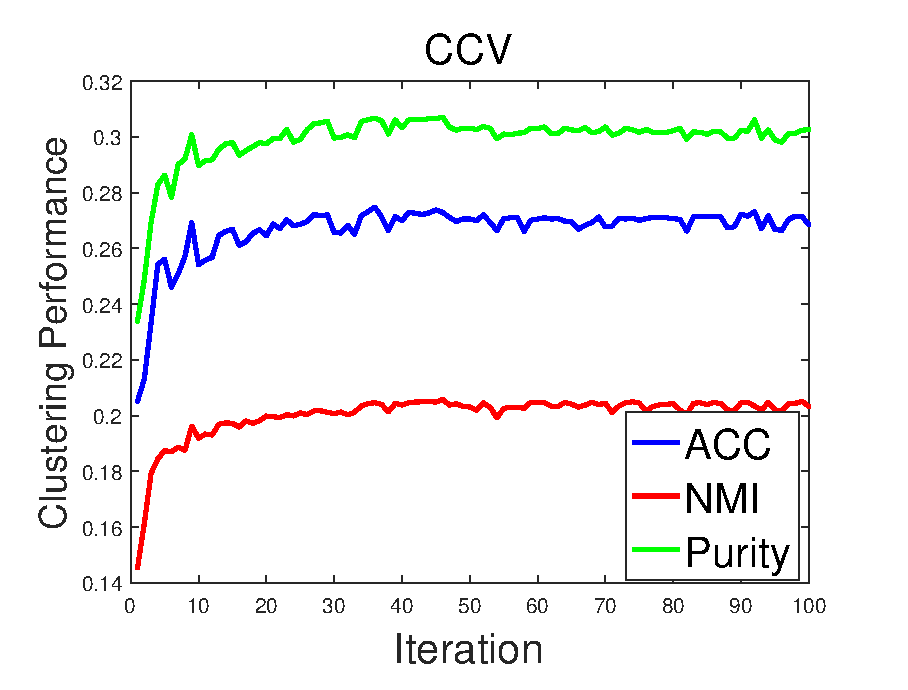
\includegraphics[width=0.5\textwidth]{figures/clusteringpictures.eps}} \label{figure_clustering}}%
\subfloat[]{{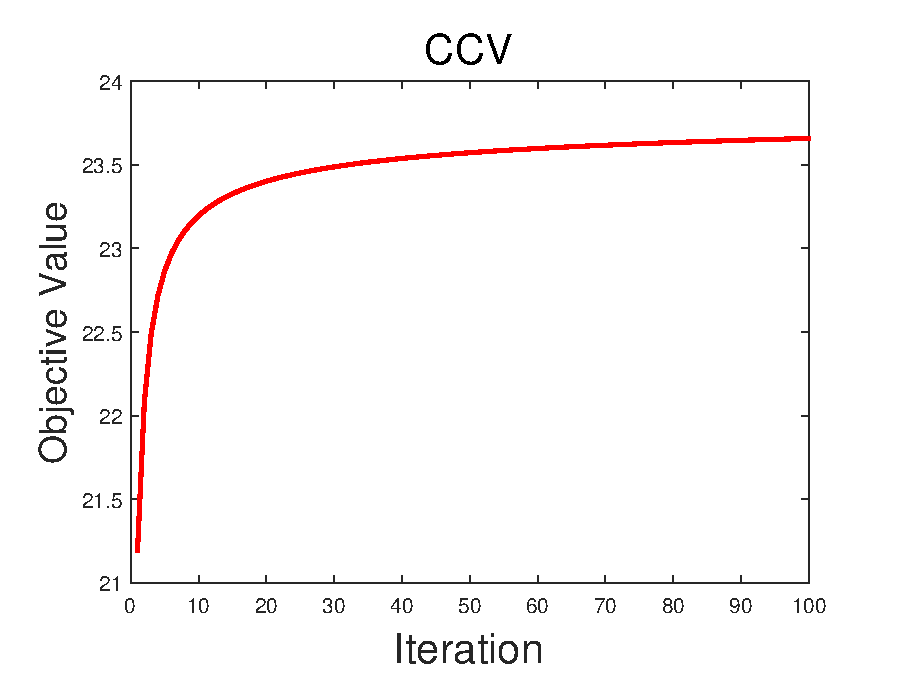
\includegraphics[width=0.5\textwidth]{figures/convergence.eps}} \label{figure_convergence}}%
\vspace{-11pt}
\caption{}
}
\end{center}
\end{figure}
    \end{itemize} 
        
\end{frame}

\begin{frame}
    \frametitle{我们的方法:MVC-LFA(Late Fusion Alignment)}
    \begin{itemize}
        \item 时间上从$\mathcal{O}(n^3)$降到了$\mathcal{O}(n)$
    \end{itemize} 
    \begin{figure}
        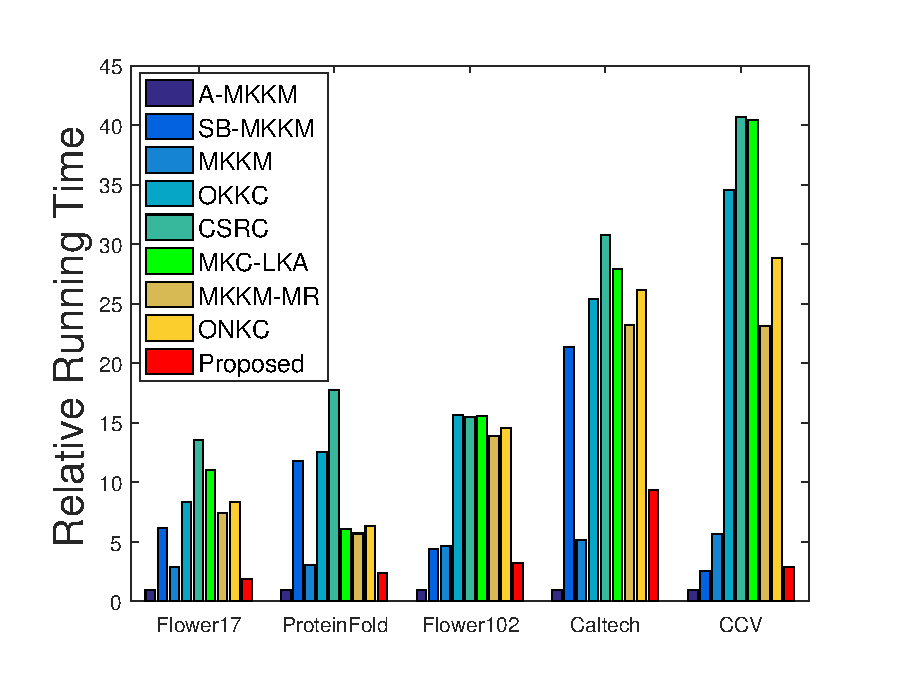
\includegraphics[width=0.8\textwidth]{figures/timepictures.eps} 
    \end{figure}          
\end{frame}
